\documentclass[aspectratio=169]{beamer}
\usetheme{Madrid}
\usecolortheme{whale}

\usepackage[T1]{fontenc}
\usepackage[utf8]{inputenc}
\usepackage{graphicx}
\usepackage{tikz}
\usepackage[siunitx]{circuitikz}
\usetikzlibrary{positioning, matrix, fit, backgrounds, shapes.callouts, tikzmark, calc, shapes.geometric, shapes.symbols}
\usepackage{pgfplots}
\pgfplotsset{compat=1.18}
\usepackage{listings}
\usepackage{booktabs}
\usepackage{hyperref}
\usepackage{amsmath}
\usepackage{xcolor}
\usepackage{minted}

\lstset{
    basicstyle=\ttfamily\tiny,
    keywordstyle=\color{blue}\bfseries,
    commentstyle=\color{gray},
    stringstyle=\color{orange},
    showstringspaces=false,
    breaklines=true,
    frame=single,
    backgroundcolor=\color{gray!10},
    language=C++,
    morekeywords={__global__, __device__, __shared__, half, float, wmma, fragment}
}

\title{GPU and Other Accelerators}
\subtitle{Performance Engineering}
\author{Technion}
\date{}

\AtBeginSection[]{
    \begin{frame}{Outline}
        \tableofcontents[currentsection]
    \end{frame}
}

\begin{document}

\begin{frame}
    \titlepage
\end{frame}

\begin{frame}{Outline}
    \tableofcontents
\end{frame}

%===============================================================================
\section{Introduction to GPGPU}
%===============================================================================

\begin{frame}{What is GPGPU?}
    \textbf{General-Purpose computing on Graphics Processing Units}

    \vspace{1em}
    \begin{columns}
        \begin{column}{0.5\textwidth}
            \textbf{Why GPUs?}
            \begin{itemize}
                \item Massive parallelism
                \item High memory bandwidth
                \item Energy efficiency
                \item Specialized units (Tensor cores)
            \end{itemize}
        \end{column}
        \begin{column}{0.5\textwidth}
            \textbf{Suitable Workloads:}
            \begin{itemize}
                \item Data-parallel algorithms (linear algebra, FFTs)
                \item Embarrassingly parallel tasks (Monte Carlo)
                \item Image/video processing
                \item AI/ML inference and training
            \end{itemize}
        \end{column}
    \end{columns}

    \vspace{1em}
    \textbf{Mature Ecosystem:}
    \begin{itemize}
        \item APIs: CUDA, OpenCL
        \item Libraries: cuBLAS, cuDNN, Thrust
        \item Frameworks: TensorFlow, PyTorch
    \end{itemize}
\end{frame}

\begin{frame}{When to Use GPU?}
    \textbf{Arithmetic Intensity:}
    \[
    I = \frac{\text{FLOPs}}{\text{bytes accessed}}
    \]

    \begin{itemize}
        \item $I \gtrsim 5$--$10$ FLOP/byte $\rightarrow$ Almost certainly \alert{compute-bound}
        \item Also known as ``Operational Intensity''
    \end{itemize}

    \vspace{1em}
    \textbf{Can still benefit with low AI:}
    \begin{itemize}
        \item Massive parallelism hides latency
        \item High-throughput HBM memory
        \item Overlap of compute \& memory operations
    \end{itemize}
\end{frame}

\begin{frame}{Roofline Model}
    Visual model for estimating performance of compute kernels.

    \begin{columns}
        \begin{column}{0.35\textwidth}
            \textbf{Key Components:}
            \begin{itemize}
                \item Maximum performance ($\pi$)
                \item Arithmetic intensity ($I$)
                \item Memory bandwidth ($\beta$)
            \end{itemize}

            \textbf{Performance bound:}
            \[
            P = \min\left\{ \pi, \; \beta \cdot I \right\}
            \]

            Highlights hardware limits and guides optimization priorities.
        \end{column}
        \begin{column}{0.65\textwidth}
            \begin{center}
            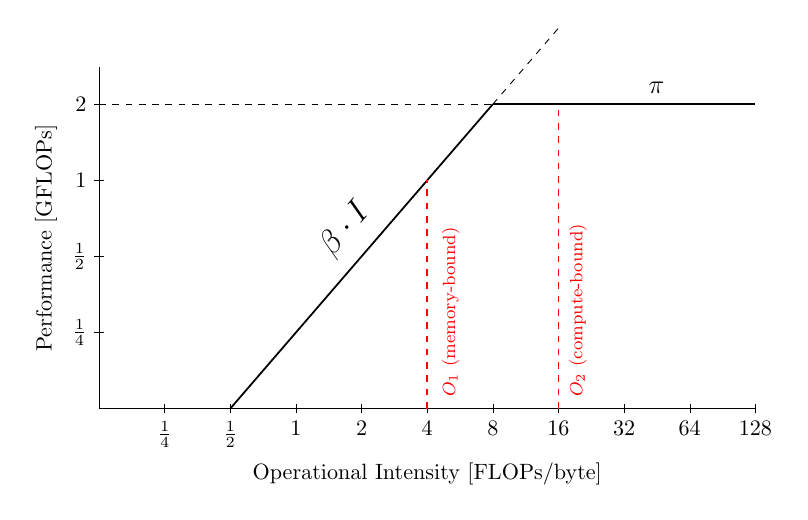
\begin{tikzpicture}[scale=0.8]
            \begin{axis}[
                name=main,
                width=12cm,
                height=7cm,
                xmode=log,
                ymode=log,
                log basis x=2,
                log basis y=2,
                xmin=0.125, xmax=128,
                ymin=0.125, ymax=2.8,
                xlabel={Operational Intensity [FLOPs/byte]},
                ylabel={Performance [GFLOPs]},
                xtick={0.25, 0.5, 1, 2, 4, 8, 16, 32, 64, 128},
                xticklabels={$\frac{1}{4}$, $\frac{1}{2}$, 1, 2, 4, 8, 16, 32, 64, 128},
                ytick={0.25, 0.5, 1, 2},
                yticklabels={$\frac{1}{4}$, $\frac{1}{2}$, 1, 2},
                axis lines=left,
                axis line style={-},
                tick style={black},
                grid=none,
                clip=false,
            ]
            % Dashed horizontal line behind pi
            \addplot[black, dashed, thin, domain=0.125:8, samples=2] {2};
            % Diagonal line (memory-bound): P = beta * I
            \addplot[black, thick, domain=0.5:8, samples=2] {0.25*x};
            % Horizontal line (compute-bound): P = pi = 2
            \addplot[black, thick, domain=8:128, samples=2] {2};
            % Dashed extension of diagonal beyond ridge
            \addplot[black, dashed, thin, domain=8:16, samples=2] {0.25*x};
            % Vertical dashed line O_1 (memory-bound)
            \addplot[red, dashed, thick] coordinates {(4, 0.125) (4, 1)};
            % Vertical dashed line O_2 (compute-bound)
            \addplot[red, dashed, thick] coordinates {(16, 0.125) (16, 2)};
            % Labels
            \node[red, rotate=90, anchor=north west, font=\footnotesize] at (axis cs:4.3,0.13) {$O_1$ (memory-bound)};
            \node[red, rotate=90, anchor=north west, font=\footnotesize] at (axis cs:16.5,0.13) {$O_2$ (compute-bound)};
            \node[anchor=south, font=\large] at (axis cs:45,2.05) {$\pi$};
            \path (axis cs:0.5,0.125) coordinate (A);
            \path (axis cs:8,2) coordinate (B);
            \end{axis}
            % Beta label with calculated angle
            \pgfmathanglebetweenpoints{\pgfpointanchor{A}{center}}{\pgfpointanchor{B}{center}}
            \let\betaangle\pgfmathresult
            \node[rotate=\betaangle, anchor=south, font=\large] at ($(A)!0.35!(B) + (-0.5,0.15)$) {$\beta \cdot I$};
            \end{tikzpicture}
            \end{center}
        \end{column}
    \end{columns}
\end{frame}

%===============================================================================
\section{GPU Architecture}
%===============================================================================

\begin{frame}{NVIDIA Blackwell Ultra --- Full Chip}
    \begin{center}
    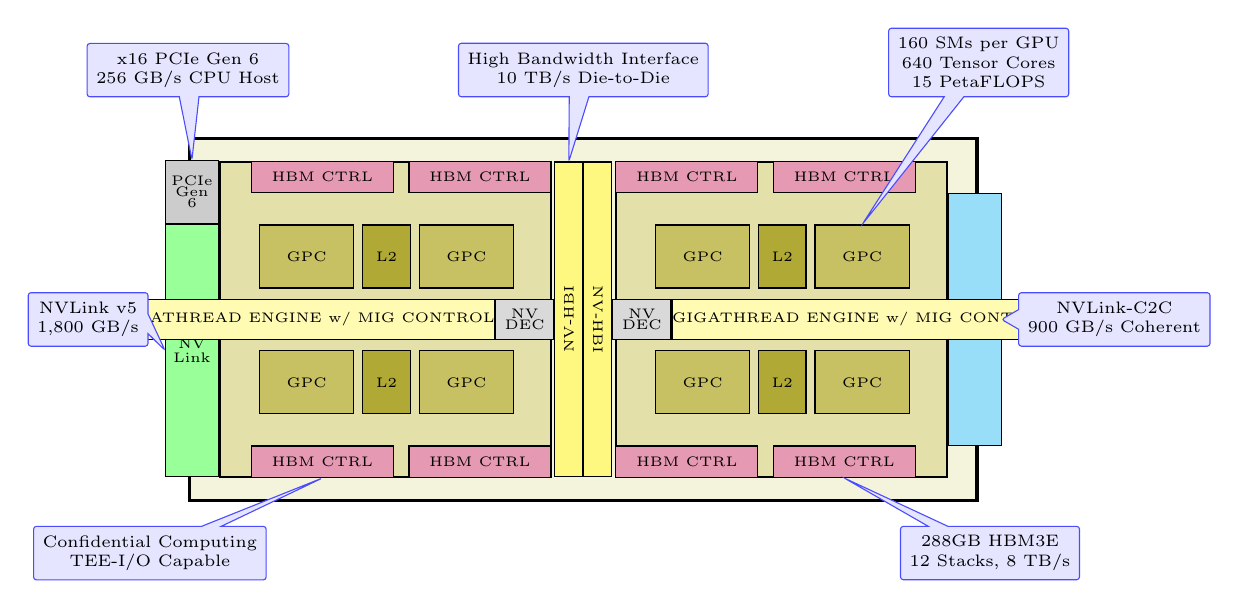
\begin{tikzpicture}[
        % Styles
        gpu/.style={draw, very thick, fill=olive!10, minimum width=100mm, minimum height=46mm},
        die/.style={draw, thick, fill=olive!25, minimum width=42mm, minimum height=40mm},
        hbm/.style={draw, fill=purple!40, minimum width=18mm, minimum height=4mm, font=\fontsize{4}{5}\selectfont, align=center},
        gpc/.style={draw, fill=olive!50, minimum width=12mm, minimum height=8mm, font=\fontsize{5}{6}\selectfont, align=center},
        l2/.style={draw, fill=olive!70, minimum width=6mm, minimum height=8mm, font=\fontsize{5}{6}\selectfont, align=center},
        engine/.style={draw, fill=yellow!30, minimum width=32mm, minimum height=5mm, font=\fontsize{4}{5}\selectfont, align=center},
        nvdec/.style={draw, fill=gray!30, minimum width=4mm, minimum height=5mm, font=\fontsize{3}{4}\selectfont, align=center},
        nvlinkbar/.style={draw, fill=green!40, text width=6mm, minimum height=32mm, font=\fontsize{4}{5}\selectfont, align=center, inner sep=1pt},
        hbi/.style={draw, fill=yellow!50, minimum width=3mm, minimum height=40mm, font=\fontsize{5}{6}\selectfont, align=center},
        pcie/.style={draw, fill=gray!40, text width=6mm, minimum height=8mm, font=\fontsize{3}{4}\selectfont, align=center, inner sep=1pt},
        callout/.style={rectangle callout, draw=blue!70, fill=blue!10, font=\fontsize{6}{7}\selectfont, align=center, rounded corners=1pt},
    ]
        % === GPU (outer rectangle) ===
        \node[gpu] (gpu) {};

        % === Two dies inside GPU ===
        \node[die, anchor=east] (dieL) at ([xshift=-4mm]gpu.center) {};
        \node[die, anchor=west] (dieR) at ([xshift=4mm]gpu.center) {};

        % === High Bandwidth Interface between dies (two narrow bars) ===
        \node[hbi, anchor=east] (hbiL) at (gpu.center) {\rotatebox{90}{NV-HBI}};
        \node[hbi, anchor=west] (hbiR) at (gpu.center) {\rotatebox{-90}{NV-HBI}};

        % === NVLink bar on left (positioned below PCIe) ===
        \node[nvlinkbar, anchor=north east] (nvlink) at ([yshift=-8mm]dieL.north west) {NV\\Link};

        % === NVLink-C2C bar on right ===
        \node[nvlinkbar, fill=cyan!40, anchor=west] (c2c) at (dieR.east) {NVLink\\C2C};

        % === PCIe at top of NVLink bar ===
        \node[pcie, anchor=south] (pcie) at (nvlink.north) {PCIe\\Gen\\6};

        % === LEFT DIE CONTENTS ===

        % Top HBM row: 2 controllers
        \node[hbm, anchor=north] (hbmLT0) at ([xshift=-8mm]dieL.north) {HBM CTRL};
        \node[hbm, anchor=north] (hbmLT1) at ([xshift=12mm]dieL.north) {HBM CTRL};

        % Bottom HBM row: 2 controllers
        \node[hbm, anchor=south] (hbmLB0) at ([xshift=-8mm]dieL.south) {HBM CTRL};
        \node[hbm, anchor=south] (hbmLB1) at ([xshift=12mm]dieL.south) {HBM CTRL};

        % GPCs: 2 above engine, 2 below
        \node[gpc] (gpcL0) at ([xshift=-10mm, yshift=8mm]dieL.center) {GPC};
        \node[l2, right=1mm of gpcL0] (l2L0) {L2};
        \node[gpc, right=1mm of l2L0] (gpcL1) {GPC};

        % NV DEC (west of NV-HBI)
        \node[nvdec, anchor=east] (nvdecL) at (hbiL.west) {NV\\DEC};

        % Engine: west of NV DEC, calculated width to fit between nvlink.east and nvdecL.west
        \path let \p1=(nvlink.east), \p2=(nvdecL.west) in
            node[engine, minimum width={\x2-\x1}, anchor=east, inner sep=0pt] (engineL) at (nvdecL.west) {GIGATHREAD ENGINE w/ MIG CONTROL};

        % GPCs below engine
        \node[gpc] (gpcL2) at ([xshift=-10mm, yshift=-8mm]dieL.center) {GPC};
        \node[l2, right=1mm of gpcL2] (l2L1) {L2};
        \node[gpc, right=1mm of l2L1] (gpcL3) {GPC};


        % === RIGHT DIE CONTENTS ===

        % Top HBM row: 2 controllers
        \node[hbm, anchor=north] (hbmRT0) at ([xshift=-12mm]dieR.north) {HBM CTRL};
        \node[hbm, anchor=north] (hbmRT1) at ([xshift=8mm]dieR.north) {HBM CTRL};

        % Bottom HBM row: 2 controllers
        \node[hbm, anchor=south] (hbmRB0) at ([xshift=-12mm]dieR.south) {HBM CTRL};
        \node[hbm, anchor=south] (hbmRB1) at ([xshift=8mm]dieR.south) {HBM CTRL};

        % GPCs: 2 above engine, 2 below
        \node[gpc] (gpcR0) at ([xshift=-10mm, yshift=8mm]dieR.center) {GPC};
        \node[l2, right=1mm of gpcR0] (l2R0) {L2};
        \node[gpc, right=1mm of l2R0] (gpcR1) {GPC};

        % NV DEC (east of NV-HBI)
        \node[nvdec, anchor=west] (nvdecR) at (hbiR.east) {NV\\DEC};

        % Engine: calculated width to fit between nvdecR.east and c2c.west
        \path let \p1=(nvdecR.east), \p2=(c2c.west) in
            node[engine, minimum width={\x2-\x1}, anchor=west, inner sep=0pt] (engineR) at (nvdecR.east) {GIGATHREAD ENGINE w/ MIG CONTROL};

        % GPCs below engine
        \node[gpc] (gpcR2) at ([xshift=-10mm, yshift=-8mm]dieR.center) {GPC};
        \node[l2, right=1mm of gpcR2] (l2R1) {L2};
        \node[gpc, right=1mm of l2R1] (gpcR3) {GPC};

        % === CALLOUTS ===
        \node[callout, callout absolute pointer={(pcie.north)}, anchor=south] at ([yshift=5mm]gpu.north west) {x16 PCIe Gen 6\\256 GB/s CPU Host};

        \node[callout, callout absolute pointer={(hbiL.north)}, anchor=south] at ([yshift=5mm]gpu.north) {High Bandwidth Interface\\10 TB/s Die-to-Die};

        \node[callout, callout absolute pointer={(gpcR1.north)}, anchor=south] at ([yshift=5mm]gpu.north east) {160 SMs per GPU\\640 Tensor Cores\\15 PetaFLOPS};

        \node[callout, callout absolute pointer={(nvlink.west)}, anchor=east] at ([xshift=-5mm]gpu.west) {NVLink v5\\1,800 GB/s};

        \node[callout, callout absolute pointer={(c2c.east)}, anchor=west] at ([xshift=5mm]gpu.east) {NVLink-C2C\\900 GB/s Coherent};

        \node[callout, callout absolute pointer={(hbmLB0.south)}, anchor=north east] at ([xshift=10mm, yshift=-3mm]gpu.south west) {Confidential Computing\\TEE-I/O Capable};

        \node[callout, callout absolute pointer={(hbmRB1.south)}, anchor=north west] at ([xshift=-10mm, yshift=-3mm]gpu.south east) {288GB HBM3E\\12 Stacks, 8 TB/s};

    \end{tikzpicture}
    \end{center}
\end{frame}

\begin{frame}<0>{NVIDIA Blackwell Ultra --- Full Chip (Original)}
    \begin{center}
        \includegraphics[height=0.85\textheight]{figures/NVIDIA-Blackwell-Ultra-GPU-chip-explained-png.png}
    \end{center}
\end{frame}

\begin{frame}{NVIDIA Blackwell Architecture (2024)}
    \textbf{NVIDIA B200 (Blackwell Architecture):}
    \begin{columns}
        \begin{column}{0.5\textwidth}
            \textbf{Top Level:}
            \begin{itemize}
                \item 208 billion transistors
                \item Dual-die design (2$\times$ GB100)
                \item 10 TB/s chip-to-chip interconnect (NV-HBI)
                \item 148 SMs
                \item 192GB HBM3e @ 8 TB/s
            \end{itemize}

            \vspace{0.5em}
            \textbf{Interconnects:}
            \begin{itemize}
                \item NVLink 5.0: 1.8 TB/s
                \item PCIe Gen5: 128 GB/s
            \end{itemize}
        \end{column}
        \begin{column}{0.5\textwidth}
            \textbf{Trends across GPU generations:}
            \begin{itemize}
                \item Tensor Cores increasingly dominant over CUDA Cores
                \item Lower precision formats (FP8 $\rightarrow$ FP4)
                \item Dedicated memory for Tensor Cores (TMEM)
                \item Multi-die designs to bypass reticle limits
                \item Memory bandwidth scaling (HBM3 $\rightarrow$ HBM3e)
            \end{itemize}
        \end{column}
    \end{columns}

    \vspace{0.3em}
    {\scriptsize Source: NVIDIA Blackwell Tuning Guide \& GTC 2024}
\end{frame}

\begin{frame}{NVIDIA Blackwell Ultra --- SM Architecture}
    \begin{columns}[T]
        \begin{column}{0.6\textwidth}
            \vspace{-0.5em}
            \textbf{Per SM (Streaming Multiprocessor):}
            \begin{itemize}
                \item 128 FP32 CUDA Cores
                \item 4 Gen5 Tensor Cores
                \item 4 Warp Schedulers (64 warps max)
            \end{itemize}

            \vspace{0.5em}
            \textbf{On-Chip Memory per SM:}
            \begin{itemize}
                \item 256KB Register File
                \item 228KB Shared Memory / L1 Cache
                \item 256KB Tensor Memory (TMEM)
            \end{itemize}

            \vspace{0.5em}
            \textbf{Memory Hierarchy:}
            \begin{itemize}
                \item \textbf{Per Thread:} Registers (max 255)
                \item \textbf{Per Block:} Shared Memory
                \item \textbf{All SMs:} L2 Cache, Global Memory
            \end{itemize}
        \end{column}
        \begin{column}{0.35\textwidth}
            \vspace{-1em}
            \begin{center}
                \includegraphics[width=\textwidth]{figures/Blackwell-Ultra-SM-architecture-png.png}
            \end{center}
        \end{column}
    \end{columns}
\end{frame}

\begin{frame}{CUDA Compilation}
    \begin{center}
    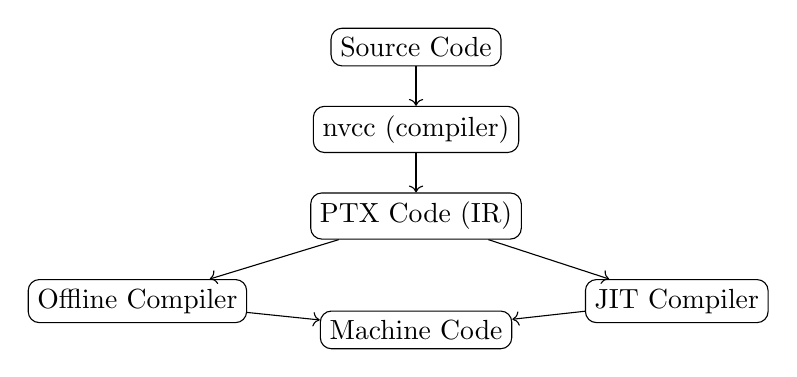
\begin{tikzpicture}[
        node distance=0.5cm and 0.8cm,
        box/.style={draw, rounded corners},
    ]
        % Vertical flow
        \node[box] (src) {Source Code};
        \node[box, below=of src] (nvcc) {nvcc (compiler)};
        \node[box, below=of nvcc] (ptx) {PTX Code (IR)};
        % Two branches from PTX
        \node[box, below left=of ptx] (offline) {Offline Compiler};
        \node[box, below right=of ptx] (jit) {JIT Compiler};
        % Final output
        \node[box, below=0.9cm of ptx] (machine) {Machine Code};

        \draw[->] (src) -- (nvcc);
        \draw[->] (nvcc) -- (ptx);
        \draw[->] (ptx) -- (offline);
        \draw[->] (ptx) -- (jit);
        \draw[->] (offline) -- (machine);
        \draw[->] (jit) -- (machine);
    \end{tikzpicture}
    \end{center}

    \begin{itemize}
        \item PTX: Intermediate representation (resembles GPU instruction set)
        \item GPU peculiarities hidden from programmer
        \item Use PTX intrinsics for performance
    \end{itemize}
\end{frame}

%===============================================================================
\section{GPU Compute}
%===============================================================================

\begin{frame}{CUDA Execution Model}
    \begin{columns}
        \begin{column}{0.5\textwidth}
            \textbf{Hierarchy (software $\rightarrow$ hardware):}
            \begin{description}
                \item[Thread] Single execution unit; has private registers
                \item[Warp] 32 threads executing in lockstep (SIMT)
                \item[Thread Block] Group of threads that can cooperate via shared memory; mapped to one SM
                \item[Grid] Collection of blocks executing same kernel
            \end{description}

            \vspace{0.5em}
            \textbf{Hardware Mapping:}
            \begin{description}
                \item[SM] Streaming Multiprocessor; executes one or more blocks concurrently
                \item[GPU] Contains many SMs (e.g., 148 on B200)
            \end{description}
        \end{column}
        \begin{column}{0.5\textwidth}
            \begin{center}
            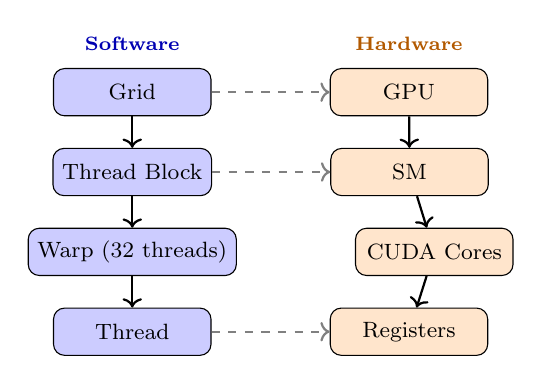
\begin{tikzpicture}[
                box/.style={draw, rounded corners, minimum width=20mm, minimum height=6mm, font=\footnotesize},
                sw/.style={box, fill=blue!20},
                hw/.style={box, fill=orange!20},
                arr/.style={->, thick},
            ]
                % Software side
                \node[sw] (grid) {Grid};
                \node[sw, below=4mm of grid] (block) {Thread Block};
                \node[sw, below=4mm of block] (warp) {Warp (32 threads)};
                \node[sw, below=4mm of warp] (thread) {Thread};

                \draw[arr] (grid) -- (block);
                \draw[arr] (block) -- (warp);
                \draw[arr] (warp) -- (thread);

                % Hardware side
                \node[hw, right=15mm of grid] (gpu) {GPU};
                \node[hw, right=15mm of block] (sm) {SM};
                \node[hw, right=15mm of warp] (cores) {CUDA Cores};
                \node[hw, right=15mm of thread] (regs) {Registers};

                \draw[arr] (gpu) -- (sm);
                \draw[arr] (sm) -- (cores);
                \draw[arr] (cores) -- (regs);

                % Mapping arrows
                \draw[arr, dashed, gray] (grid) -- (gpu);
                \draw[arr, dashed, gray] (block) -- (sm);
                \draw[arr, dashed, gray] (thread) -- (regs);

                % Labels
                \node[above=1mm of grid, font=\scriptsize\bfseries, blue!70!black] {Software};
                \node[above=1mm of gpu, font=\scriptsize\bfseries, orange!70!black] {Hardware};
            \end{tikzpicture}
            \end{center}
        \end{column}
    \end{columns}

    \vspace{0.3em}
    {\scriptsize Source: CUDA C++ Programming Guide}
\end{frame}

\begin{frame}[fragile]{SM Architecture \& Warp Scheduling}
\begin{center}
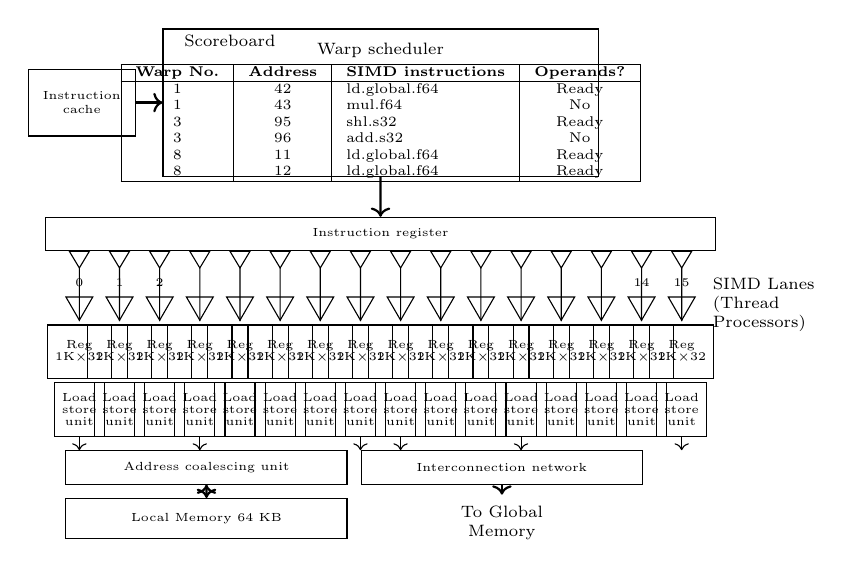
\begin{tikzpicture}[scale=0.85, every node/.style={font=\tiny, transform shape},
    box/.style={draw, fill=#1, minimum height=7mm, align=center},
    box/.default=white,
    lane/.style={draw, minimum width=6mm, minimum height=5mm, align=center, font=\fontsize{4}{5}\selectfont},
    alu/.style={draw, fill=white, isosceles triangle, isosceles triangle apex angle=60,
                shape border rotate=-90, minimum width=4mm, minimum height=3mm, inner sep=0pt},
]

% Instruction cache
\node[box, minimum width=16mm, minimum height=10mm] (icache) at (0,0) {Instruction\\cache};

% Warp scheduler box with scoreboard
\node[box, minimum width=65mm, minimum height=22mm, anchor=west]
    (scheduler) at ([xshift=4mm]icache.east) {};
\node[anchor=north, font=\scriptsize] at ([yshift=-1mm]scheduler.north) {Warp scheduler};

% Scoreboard table
\node[anchor=north, yshift=-4mm] at (scheduler.north) {
\fontsize{6}{7}\selectfont
\begin{tabular}{|c|c|l|c|}
\hline
\textbf{Warp No.} & \textbf{Address} & \textbf{SIMD instructions} & \textbf{Operands?} \\
\hline
1 & 42 & ld.global.f64 & Ready \\
1 & 43 & mul.f64 & No \\
3 & 95 & shl.s32 & Ready \\
3 & 96 & add.s32 & No \\
8 & 11 & ld.global.f64 & Ready \\
8 & 12 & ld.global.f64 & Ready \\
\hline
\end{tabular}
};
\node[anchor=south west, font=\scriptsize] at ([xshift=2mm, yshift=-4mm]scheduler.north west) {Scoreboard};

% Arrow from instruction cache to scheduler
\draw[->, thick] (icache.east) -- (scheduler.west);

% Instruction register as rectangle
\node[box, minimum width=100mm, minimum height=5mm, anchor=north]
    (ireg) at ([yshift=-6mm]scheduler.south) {Instruction register};

% Arrow from scheduler to instruction register
\draw[->, thick] (scheduler.south) -- (ireg.north);

% Draw triangular pins below instruction register and 16 SIMD lanes
\foreach \i in {0,...,15} {
    % Calculate x position for this lane
    \coordinate (pin\i) at ([xshift=\i*6mm-45mm]ireg.south);

    % Draw triangular pin marker
    \draw[fill=white] (pin\i) -- ++(-1.5mm,0) -- ++(1.5mm,-2.5mm) -- ++(1.5mm,2.5mm) -- cycle;

    % ALU triangle below the pin
    \node[alu] (alu\i) at ([yshift=-8mm]pin\i) {};

    % Registers box with size inside
    \node[lane, anchor=north, minimum height=8mm] at ([yshift=-0.5mm]alu\i.south) (reg\i) {Reg\\{\fontsize{3}{4}\selectfont 1K$\times$32}};

    % Load store unit
    \node[lane, anchor=north, minimum height=8mm] at ([yshift=-0.5mm]reg\i.south) (lsu\i) {Load\\store\\unit};

    % Connect pin to ALU
    \draw ([yshift=-2.5mm]pin\i) -- (alu\i.apex);
}

% Lane labels (only show a few) - black text
\node[font=\fontsize{5}{6}\selectfont] at ([yshift=2mm]alu0.north) {0};
\node[font=\fontsize{5}{6}\selectfont] at ([yshift=2mm]alu1.north) {1};
\node[font=\fontsize{5}{6}\selectfont] at ([yshift=2mm]alu2.north) {2};
\node[font=\fontsize{5}{6}\selectfont] at ([yshift=2mm]alu14.north) {14};
\node[font=\fontsize{5}{6}\selectfont] at ([yshift=2mm]alu15.north) {15};

% SIMD Lanes label
\node[anchor=west, font=\scriptsize, align=left] at ([xshift=2mm]alu15.east)
    {SIMD Lanes\\(Thread\\Processors)};

% Address coalescing unit
\node[box, minimum width=42mm, minimum height=5mm, anchor=north]
    (coalesce) at ([yshift=-2mm, xshift=-23mm]lsu7.south) {Address coalescing unit};

% Interconnection network
\node[box, minimum width=42mm, minimum height=5mm, anchor=north west]
    (interconnect) at ([xshift=2mm]coalesce.north east) {Interconnection network};

% Arrows from lanes to bottom units
\foreach \i in {0,3,7} {
    \draw[->, thin] (lsu\i.south) -- (lsu\i.south |- coalesce.north);
}
\foreach \i in {8,11,15} {
    \draw[->, thin] (lsu\i.south) -- (lsu\i.south |- interconnect.north);
}

% Local memory
\node[box, minimum width=42mm, minimum height=6mm, anchor=north]
    (localmem) at ([yshift=-2mm]coalesce.south) {Local Memory 64 KB};

% Arrow between coalescing and local memory
\draw[<->, thick] (coalesce.south) -- (localmem.north);

% To global memory
\node[anchor=north, font=\scriptsize, align=center] at ([yshift=-2mm]interconnect.south)
    {To Global\\Memory};
\draw[->, thick] (interconnect.south) -- ++(0,-1.5mm);

\end{tikzpicture}
\end{center}
\end{frame}
\begin{frame}{GPU Scheduler}
    \textbf{Grid \& Block Dispatch:}
    \begin{itemize}
        \item Kernel $\rightarrow$ grid of blocks
        \item SMs pull blocks when resources available
    \end{itemize}

    \vspace{0.5em}
    \textbf{Warp Scheduling:}
    \begin{itemize}
        \item Threads grouped into 32-thread \textbf{warps}
        \item Warp scheduler issues ready warps to hide stalls
        \item \textbf{Occupancy} = $\frac{\text{active warps}}{\text{max warps per SM}}$
    \end{itemize}

    \vspace{0.5em}
    \textbf{Latency Hiding:}
    \begin{itemize}
        \item High occupancy $\Rightarrow$ many warps queued
        \item When one warp stalls (memory), another executes
    \end{itemize}

    \vspace{0.5em}
    \textbf{Tune for Balance:}
    \begin{itemize}
        \item Choose block size to maximize occupancy
        \item Limit registers/thread to avoid spills
    \end{itemize}
\end{frame}

\begin{frame}{Registers}
    \textbf{Limited On-Chip Resource:}
    \begin{itemize}
        \item Each SM has fixed register file (e.g., 64K registers)
        \item Each thread can use at most 255 registers
    \end{itemize}

    \vspace{0.5em}
    \textbf{Trade-off:}
    \begin{itemize}
        \item Registers per thread cap number of resident warps
        \item High occupancy helps hide memory latency
        \item Excessive register use improves ILP but may starve SM
    \end{itemize}

    \vspace{0.5em}
    \textbf{Tuning:}
    \begin{itemize}
        \item Use \texttt{-maxrregcount} or \texttt{\_\_launch\_bounds\_\_()} to limit registers
        \item \textbf{Register spilling}: 100s of cycles penalty
        \item Refactor code to reuse variables and reduce live ranges
    \end{itemize}
\end{frame}

\begin{frame}{GPU Warp Divergence}
    \textbf{Problem:} Conditional branches cause threads within a warp to diverge.

    \begin{itemize}
        \item All 32 threads in a warp share \textbf{one Program Counter}
        \item When threads take different paths, execution is \textbf{serialized}
        \item Hardware uses an \textbf{active mask} to track which threads execute
        \item PC and mask are pushed onto a \textbf{stack} at each branch
    \end{itemize}

    \vspace{1em}
    \textbf{Convergence:} When both paths complete, threads merge back and all become active again.

    \vspace{1em}
    \textbf{Performance Impact:}
    \begin{itemize}
        \item Divergent warps take time proportional to \textbf{sum of all paths}
        \item Worst case: 32$\times$ slowdown if every thread takes a different path
        \item Nested branches compound the problem
    \end{itemize}

    \vspace{1em}
    \textbf{Mitigation strategies:} Data reorganization, predicated instructions, separate kernels, warp-level primitives
\end{frame}

\begin{frame}[fragile]{GPU Warp Divergence: Example}
\begin{columns}
\begin{column}{0.45\textwidth}
\begin{lstlisting}[language=C, basicstyle=\ttfamily\small, numbers=left, numberstyle=\tiny, xleftmargin=2em, backgroundcolor={}, escapechar=|]
int tid = threadIdx.x;
if (tid < 4) {
    |\tikzmark{L3s}|foo();|\tikzmark{L3e}|
    if (tid < 2) {
        |\tikzmark{L5s}|bar();|\tikzmark{L5e}|
    } else {
        |\tikzmark{L7s}|baz();|\tikzmark{L7e}|
    }
} else {
    |\tikzmark{L10s}|qux();|\tikzmark{L10e}|
}
|\tikzmark{L12s}|// All converge|\tikzmark{L12e}|
\end{lstlisting}
\end{column}

\begin{column}{0.5\textwidth}
\begin{tikzpicture}[scale=0.92,
    active/.style={draw, fill=green!40, minimum width=5mm, minimum height=4.5mm, font=\scriptsize},
    inactive/.style={draw, fill=white, minimum width=5mm, minimum height=4.5mm, font=\scriptsize},
    steplbl/.style={font=\scriptsize\bfseries, anchor=south west, yshift=-3mm},
    dots/.style={font=\scriptsize, minimum width=5mm},
]

% Stage 1: Callout explaining tid = thread index (with proper TikZ callout shape)
\only<1>{
\node[rectangle callout, callout relative pointer={(-5cm, 2cm)}, draw, fill=blue!10,
      font=\scriptsize, align=left, text width=4cm] (tidcallout) at (2, -2) {
    \textbf{tid} = thread index (0--31)\\[2pt]
    Each box shows thread's \textbf{tid}\\[2pt]
    Thread 0 has tid=0, thread 1 has tid=1, etc.
};
}

% Stage 2: Step 1 - All 32 Threads Active
\only<2->{
\matrix[matrix of nodes, row sep=0pt, column sep=1pt, anchor=north west, ampersand replacement=\&] (s1) at (0,0) {
    |[active]| 0 \& |[active]| 1 \& |[active]| 2 \& |[active]| 3 \&
    |[active]| 4 \& |[active]| 5 \& |[active]| 6 \& |[active]| 7 \& |[dots]| \ldots{} 31 \\
};
\node[steplbl] at (s1.north west) {Step 1: All 32 Threads Active};
}

% Stage 3: Step 2 - x = qux() for tid < 4
\only<3->{
\matrix[matrix of nodes, row sep=0pt, column sep=1pt, anchor=north west, ampersand replacement=\&] (s2) at (0,-1.1) {
    |[active]| 0 \& |[active]| 1 \& |[active]| 2 \& |[active]| 3 \&
    |[inactive]| 4 \& |[inactive]| 5 \& |[inactive]| 6 \& |[inactive]| 7 \& |[dots]| \ldots \\
};
\node[steplbl] at (s2.north west) {Step 2: foo()};
}

% Stage 4: Step 3 - bar() for tid < 2
\only<4->{
\matrix[matrix of nodes, row sep=0pt, column sep=1pt, anchor=north west, ampersand replacement=\&] (s3) at (0,-2.2) {
    |[active]| 0 \& |[active]| 1 \& |[inactive]| 2 \& |[inactive]| 3 \&
    |[inactive]| 4 \& |[inactive]| 5 \& |[inactive]| 6 \& |[inactive]| 7 \& |[dots]| \ldots \\
};
\node[steplbl] at (s3.north west) {Step 3: bar()};
}

% Stage 5: Step 4 - baz() for 2 <= tid < 4
\only<5->{
\matrix[matrix of nodes, row sep=0pt, column sep=1pt, anchor=north west, ampersand replacement=\&] (s4) at (0,-3.3) {
    |[inactive]| 0 \& |[inactive]| 1 \& |[active]| 2 \& |[active]| 3 \&
    |[inactive]| 4 \& |[inactive]| 5 \& |[inactive]| 6 \& |[inactive]| 7 \& |[dots]| \ldots \\
};
\node[steplbl] at (s4.north west) {Step 4: baz()};
}

% Stage 6: Step 5 - qux() for tid >= 4
\only<6->{
\matrix[matrix of nodes, row sep=0pt, column sep=1pt, anchor=north west, ampersand replacement=\&] (s5) at (0,-4.4) {
    |[inactive]| 0 \& |[inactive]| 1 \& |[inactive]| 2 \& |[inactive]| 3 \&
    |[active]| 4 \& |[active]| 5 \& |[active]| 6 \& |[active]| 7 \& |[dots]| \ldots \\
};
\node[steplbl] at (s5.north west) {Step 5: qux()};
}

% Stage 7: Step 6 - Convergence
\only<7>{
\matrix[matrix of nodes, row sep=0pt, column sep=1pt, anchor=north west, ampersand replacement=\&] (s6) at (0,-5.5) {
    |[active]| 0 \& |[active]| 1 \& |[active]| 2 \& |[active]| 3 \&
    |[active]| 4 \& |[active]| 5 \& |[active]| 6 \& |[active]| 7 \& |[dots]| \ldots{} 31 \\
};
\node[steplbl, text=green!50!black] at (s6.north west) {Step 6: Convergence};
}

% Legend (show from stage 2 onwards) - moved lower by 8mm and right by 1cm
\only<2->{
\node[active, label=right:{\scriptsize Active}] at (1,-7.3) {};
\node[inactive, label=right:{\scriptsize Inactive (masked)}] at (3,-7.3) {};
}

\end{tikzpicture}
\end{column}
\end{columns}

% Code highlighting overlay using tikzmarks - yellow background with blend mode

\begin{tikzpicture}[remember picture, overlay]
    \begin{scope}[blend mode=multiply]
    % Stage 3: highlight "foo();" - runs for all tid < 4
    \only<3>{
        \fill[yellow!60, rounded corners=2pt]
            ([xshift=-2pt, yshift=9pt]pic cs:L3s) rectangle
            ([xshift=2pt, yshift=-1pt]pic cs:L3e);
    }
    % Stage 4: highlight "bar();" - runs for tid < 2
    \only<4>{
        \fill[yellow!60, rounded corners=2pt]
            ([xshift=-2pt, yshift=9pt]pic cs:L5s) rectangle
            ([xshift=2pt, yshift=-1pt]pic cs:L5e);
    }
    % Stage 5: highlight "baz();" - runs for 2 <= tid < 4
    \only<5>{
        \fill[yellow!60, rounded corners=2pt]
            ([xshift=-2pt, yshift=9pt]pic cs:L7s) rectangle
            ([xshift=2pt, yshift=-1pt]pic cs:L7e);
    }
    % Stage 6: highlight "qux();" - runs for tid >= 4
    \only<6>{
        \fill[yellow!60, rounded corners=2pt]
            ([xshift=-2pt, yshift=9pt]pic cs:L10s) rectangle
            ([xshift=2pt, yshift=-1pt]pic cs:L10e);
    }
    % Stage 7: highlight "// All converge" - all threads reconverge
    \only<7>{
        \fill[green!60, rounded corners=2pt]
            ([xshift=-2pt, yshift=9pt]pic cs:L12s) rectangle
            ([xshift=2pt, yshift=-1pt]pic cs:L12e);
    }
    \end{scope}
\end{tikzpicture}
\end{frame}
\begin{frame}[fragile]{Warp-Level Primitives Example}
    \begin{columns}
        \begin{column}{0.5\textwidth}
            \textbf{Warp reduction without divergence:}

\begin{lstlisting}[basicstyle=\ttfamily\small]
#define FULL_MASK 0xffffffff

for (int offset = 16; offset > 0; offset /= 2)
    val += __shfl_down_sync(FULL_MASK, val, offset);
\end{lstlisting}

            \textbf{Benefits:}
            \begin{itemize}
                \item No shared memory needed
                \item No synchronization barriers
                \item Efficient intra-warp communication
            \end{itemize}

            \textbf{Replace branches with arithmetic:}
\begin{lstlisting}[basicstyle=\ttfamily\small]
result = condition * trueValue
       + (!condition) * falseValue;
\end{lstlisting}
        \end{column}
        \begin{column}{0.5\textwidth}
            \begin{center}
            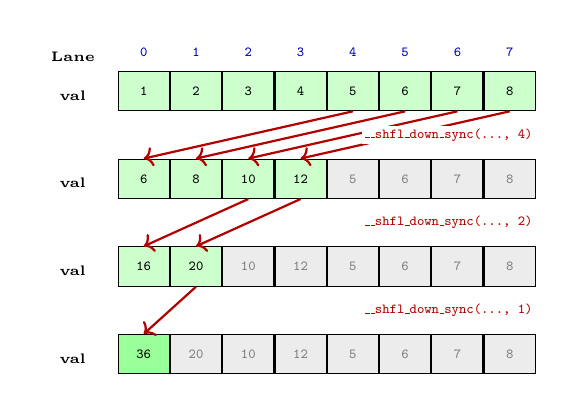
\begin{tikzpicture}[
                val/.style={draw, minimum width=6.5mm, minimum height=5mm,
                            font=\tiny\ttfamily, fill=green!20, inner sep=0pt},
                valg/.style={val, fill=gray!15, text=gray},
                hdr/.style={minimum width=6.5mm, minimum height=4mm,
                            font=\tiny\ttfamily, inner sep=0pt, text=blue!70!black},
                lbl/.style={font=\tiny\bfseries, text=black, minimum width=10mm,
                            align=right, anchor=east},
                gap/.style={minimum height=6mm, inner sep=0pt},
                arr/.style={->, thick, red!70!black},
            ]
                \matrix[matrix of nodes, column sep=0pt, row sep=0pt,
                        ampersand replacement=\&] (m) {
                    % Row 1: Lane headers
                    |[lbl]| Lane \&
                    |[hdr]| 0 \& |[hdr]| 1 \& |[hdr]| 2 \& |[hdr]| 3 \&
                    |[hdr]| 4 \& |[hdr]| 5 \& |[hdr]| 6 \& |[hdr]| 7 \\
                    % Row 2: Initial values
                    |[lbl]| val \&
                    |[val]| 1 \& |[val]| 2 \& |[val]| 3 \& |[val]| 4 \&
                    |[val]| 5 \& |[val]| 6 \& |[val]| 7 \& |[val]| 8 \\
                    % Row 3: Gap for arrows
                    |[gap]| \& |[gap]| \& |[gap]| \& |[gap]| \& |[gap]| \&
                    |[gap]| \& |[gap]| \& |[gap]| \& |[gap]| \\
                    % Row 4: After offset=4
                    |[lbl]| val \&
                    |[val]| 6 \& |[val]| 8 \& |[val]| 10 \& |[val]| 12 \&
                    |[valg]| 5 \& |[valg]| 6 \& |[valg]| 7 \& |[valg]| 8 \\
                    % Row 5: Gap for arrows
                    |[gap]| \& |[gap]| \& |[gap]| \& |[gap]| \& |[gap]| \&
                    |[gap]| \& |[gap]| \& |[gap]| \& |[gap]| \\
                    % Row 6: After offset=2
                    |[lbl]| val \&
                    |[val]| 16 \& |[val]| 20 \& |[valg]| 10 \& |[valg]| 12 \&
                    |[valg]| 5 \& |[valg]| 6 \& |[valg]| 7 \& |[valg]| 8 \\
                    % Row 7: Gap for arrows
                    |[gap]| \& |[gap]| \& |[gap]| \& |[gap]| \& |[gap]| \&
                    |[gap]| \& |[gap]| \& |[gap]| \& |[gap]| \\
                    % Row 8: Final result
                    |[lbl]| val \&
                    |[val, fill=green!40]| 36 \& |[valg]| 20 \& |[valg]| 10 \& |[valg]| 12 \&
                    |[valg]| 5 \& |[valg]| 6 \& |[valg]| 7 \& |[valg]| 8 \\
                };

                % Shuffle arrows: offset=4 (row 2 -> row 4)
                \foreach \src/\dst in {6/2, 7/3, 8/4, 9/5} {
                    \draw[arr] (m-2-\src.south) -- (m-4-\dst.north);
                }
                % Shuffle arrows: offset=2 (row 4 -> row 6)
                \foreach \src/\dst in {4/2, 5/3} {
                    \draw[arr] (m-4-\src.south) -- (m-6-\dst.north);
                }
                % Shuffle arrows: offset=1 (row 6 -> row 8)
                \draw[arr] (m-6-3.south) -- (m-8-2.north);

                % Operation annotations aligned to right edge of last value cell
                \node[font=\tiny\ttfamily, text=red!70!black, anchor=east, fill=white, inner sep=1pt]
                    at (m-2-9.east |- m-3-9) {\_\_shfl\_down\_sync(..., 4)};
                \node[font=\tiny\ttfamily, text=red!70!black, anchor=east, fill=white, inner sep=1pt]
                    at (m-2-9.east |- m-5-9) {\_\_shfl\_down\_sync(..., 2)};
                \node[font=\tiny\ttfamily, text=red!70!black, anchor=east, fill=white, inner sep=1pt]
                    at (m-2-9.east |- m-7-9) {\_\_shfl\_down\_sync(..., 1)};
            \end{tikzpicture}
            \end{center}
        \end{column}
    \end{columns}
\end{frame}

\begin{frame}{Kernel Fusion and Fission}
    \begin{columns}
        \begin{column}{0.5\textwidth}
            \textbf{Kernel Fusion:}
            \begin{itemize}
                \item Combine multiple sequential kernels into one
                \item Reduces launch overhead
                \item Reduces global memory traffic
                \item Reuse data in registers/shared memory
            \end{itemize}

            \textbf{Trade-off:}
            \begin{itemize}
                \item May increase register pressure
                \item Can limit occupancy
            \end{itemize}
        \end{column}
        \begin{column}{0.5\textwidth}
            \textbf{Kernel Fission:}
            \begin{itemize}
                \item Split large kernel into smaller ones
                \item Lowers register/shared memory usage
                \item Improves occupancy
                \item Exposes finer-grained parallelism
            \end{itemize}

            \textbf{Trade-off:}
            \begin{itemize}
                \item Extra launches
                \item Additional memory transfers
            \end{itemize}
        \end{column}
    \end{columns}
\end{frame}

\begin{frame}{DPX Instructions}
    \begin{columns}
        \begin{column}{0.55\textwidth}
            \textbf{Dynamic Programming eXtensions:}

            \begin{itemize}
                \item Specialized fused-compute instructions
                \item Find min/max values with fused addition
                \item Works on 16 and 32-bit signed/unsigned integers
                \item Optional ReLU (clamping to zero)
            \end{itemize}

            \vspace{0.5em}
            \textbf{Example: Floyd--Warshall Algorithm}

            Find shortest paths between all pairs of vertices:
            \[
            \text{dist}[i][j] = \min(\text{dist}[i][j], \text{dist}[i][k] + \text{dist}[k][j])
            \]

            DPX accelerates the \texttt{min(a, b + c)} operation.
        \end{column}
        \begin{column}{0.45\textwidth}
            \begin{center}
                \includegraphics[width=\textwidth]{figures/10-floyd-warshall-iterations.png}
            \end{center}
        \end{column}
    \end{columns}
\end{frame}

%===============================================================================
\section{Tensor Cores}
%===============================================================================

\begin{frame}{Tensor Cores}
    \begin{columns}
        \begin{column}{0.65\textwidth}
            \textbf{Specialized for matrix multiply-accumulate (MMA) operations.}

            \vspace{0.5em}
            \textbf{Tensor Cores dominate LLM workloads:}
            \begin{itemize}
                \item Transformers are \alert{matrix multiplication machines}
                \item Attention: $\text{softmax}\left(\frac{QK^T}{\sqrt{d}}\right) \cdot V$ --- all matmuls
                \item Feed-forward layers: dense matrix multiplications
                \item Single Tensor Core op: 16$\times$16$\times$16 MMA (FP16)
            \end{itemize}

            \vspace{0.5em}
            \textbf{WMMA (Warp Matrix Multiply Accumulate):}
            \begin{itemize}
                \item Used internally by cuBLAS, cuDNN, PyTorch, TensorFlow
                \item Fused multiply-add in single clock cycle
                \item GPU tiling: large matrices $\rightarrow$ small tiles in shared memory
            \end{itemize}

            \vspace{0.3em}
            \begin{block}{Key Insight}
                $>$90\% of LLM compute time is spent in Tensor Core operations.
            \end{block}
        \end{column}
        \begin{column}{0.35\textwidth}
            \vspace{-4.5em}
            \begin{center}
            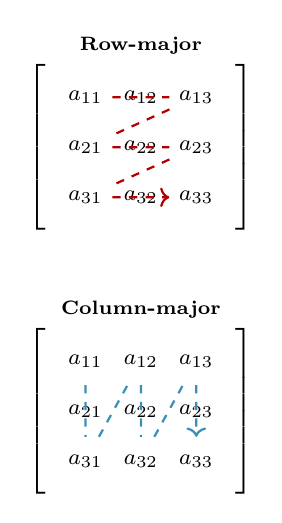
\begin{tikzpicture}[
                cell/.style={minimum size=6mm, anchor=center, font=\footnotesize},
                arr/.style={->, thick, red!70!black}]
                % Row-major
                \matrix[matrix of math nodes, nodes={cell}, row sep=1pt,
                        column sep=1pt, ampersand replacement=\&,
                        left delimiter={[}, right delimiter={]},
                        label={[font=\scriptsize\bfseries]above:Row-major}] (R) {
                    a_{11} \& a_{12} \& a_{13} \\
                    a_{21} \& a_{22} \& a_{23} \\
                    a_{31} \& a_{32} \& a_{33} \\
                };
                \draw[arr, dashed] (R-1-1) -- (R-1-3) -- (R-2-1) -- (R-2-3) -- (R-3-1) -- (R-3-3);

                % Column-major
                \matrix[matrix of math nodes, nodes={cell}, row sep=1pt,
                        column sep=1pt, ampersand replacement=\&,
                        left delimiter={[}, right delimiter={]}, below=35pt of R,
                        label={[font=\scriptsize\bfseries]above:Column-major}] (C) {
                    a_{11} \& a_{12} \& a_{13} \\
                    a_{21} \& a_{22} \& a_{23} \\
                    a_{31} \& a_{32} \& a_{33} \\
                };
                \draw[arr, cyan!70!black, dashed] (C-1-1) -- (C-3-1) -- (C-1-2) -- (C-3-2) -- (C-1-3) -- (C-3-3);
            \end{tikzpicture}
            \end{center}
        \end{column}
    \end{columns}
\end{frame}

\begin{frame}[fragile]{Tensor Cores: WMMA Example}
\begin{lstlisting}
#include <mma.h>
using namespace nvcuda;

__global__ void wmma_ker(half *a, half *b, float *c) {
   // Declare the fragments
   wmma::fragment<wmma::matrix_a, 16, 16, 16, half, wmma::col_major> a_frag;
   wmma::fragment<wmma::matrix_b, 16, 16, 16, half, wmma::row_major> b_frag;
   wmma::fragment<wmma::accumulator, 16, 16, 16, float> c_frag;

   // Initialize the output to zero
   wmma::fill_fragment(c_frag, 0.0f);

   // Load the inputs
   wmma::load_matrix_sync(a_frag, a, 16);
   wmma::load_matrix_sync(b_frag, b, 16);

   // Perform the matrix multiplication
   wmma::mma_sync(c_frag, a_frag, b_frag, c_frag);

   // Store the output
   wmma::store_matrix_sync(c, c_frag, 16, wmma::mem_row_major);
}
\end{lstlisting}
\end{frame}

\begin{frame}{Tensor Core Precisions}
    \begin{columns}
        \begin{column}{0.5\textwidth}
            \textbf{Floating-Point Formats:}
            \begin{description}
                \item[FP32] 32 bits --- full precision baseline
                \item[TF32] 19 bits --- $\sim$10$\times$ speedup, same range as FP32
                \item[FP16] 16 bits --- standard for deep learning
                \item[BF16] 16 bits --- same range as FP32, fewer mantissa bits
                \item[FP8] 8 bits --- Hopper+, 2$\times$ throughput vs FP16
                \item[FP4] 4 bits --- Blackwell, 4$\times$ throughput vs FP8
            \end{description}
        \end{column}
        \begin{column}{0.5\textwidth}
            \textbf{Integer Formats:}
            \begin{description}
                \item[INT8] Quantized inference, 4$\times$ vs FP32
                \item[INT4] Highest throughput for extreme quantization
            \end{description}

            \vspace{1em}
            \textbf{Mixed Precision Pattern:}
            \begin{itemize}
                \item Inputs: FP16/BF16/FP8/FP4
                \item Accumulator: \alert{always FP32}
                \item Maintains numerical stability
            \end{itemize}

            \vspace{0.5em}
            \begin{block}{Trend}
                Each generation adds lower precision $\rightarrow$ higher throughput.
            \end{block}
        \end{column}
    \end{columns}
\end{frame}

\begin{frame}{Tensor Memory (TMEM) --- Blackwell}
    \begin{columns}
        \begin{column}{0.5\textwidth}
            \textbf{What is TMEM?}
            \begin{itemize}
                \item 256KB dedicated on-chip memory per SM
                \item 128 lanes $\times$ 512 columns $\times$ 4 bytes
                \item Specialized for Tensor Core accumulators
                \item Separate from registers and shared memory
            \end{itemize}

            \vspace{0.5em}
            \textbf{Benefits:}
            \begin{itemize}
                \item Zero register pressure for MMA operations
                \item Decouples Tensor Cores from CUDA Cores
                \item Higher occupancy possible
            \end{itemize}
        \end{column}
        \begin{column}{0.5\textwidth}
            \textbf{Evolution of Tensor Core Data Flow:}
            \begin{enumerate}
                \item \textbf{Volta/Ampere:} Operands \& accumulators in registers
                \item \textbf{Hopper:} TMA loads operands directly to shared memory
                \item \textbf{Blackwell:} TMEM holds accumulators
            \end{enumerate}

            \vspace{0.5em}
            \textbf{Trade-offs:}
            \begin{itemize}
                \item Must explicitly manage TMEM allocation
                \item Custom ops on accumulators require TMEM $\leftrightarrow$ register copies
                \item Restricted access patterns (warpgroup-based)
            \end{itemize}
        \end{column}
    \end{columns}
\end{frame}

\begin{frame}<0>{Quantization}  % Hidden slide
    \textbf{Software technique: converting high-precision weights to lower-precision formats.}

    \begin{columns}
        \begin{column}{0.5\textwidth}
            \textbf{Benefits:}
            \begin{itemize}
                \item Lower memory footprint
                \item Faster inference (Tensor Cores accelerate INT8/INT4/FP8/FP4)
                \item Enables deployment on resource-constrained hardware
            \end{itemize}

            \vspace{0.5em}
            \textbf{Common Schemes:}
            \begin{description}
                \item[PTQ] Post-Training Quantization --- quantize after training
                \item[QAT] Quantization-Aware Training --- simulate quantization during training
            \end{description}
        \end{column}
        \begin{column}{0.5\textwidth}
            \textbf{Connection to Hardware:}
            \begin{itemize}
                \item FP32 model $\rightarrow$ INT8 weights = 4$\times$ smaller
                \item Tensor Cores have dedicated INT8/INT4 datapaths
                \item Mixed precision: INT8 compute, FP32 accumulator
            \end{itemize}

            \vspace{0.5em}
            \begin{alertblock}{Trade-off}
                Potential accuracy loss --- must validate on your workload.
            \end{alertblock}
        \end{column}
    \end{columns}
\end{frame}

%===============================================================================
\section{GPU Memory}
%===============================================================================

\begin{frame}{GPU Memory Hierarchy}
    \begin{columns}
        \begin{column}{0.45\textwidth}
            \textbf{B200 Memory Hierarchy:}
            \begin{center}
            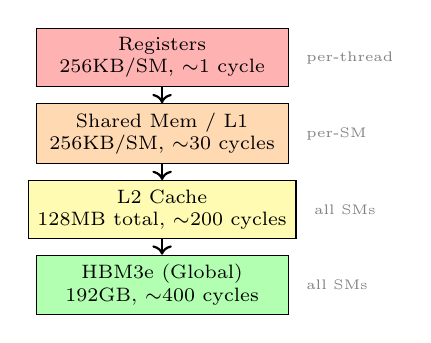
\begin{tikzpicture}[
                level/.style={draw, minimum width=32mm, minimum height=7mm, font=\scriptsize, align=center},
                arr/.style={->, thick},
            ]
                \node[level, fill=red!30] (reg) {Registers\\256KB/SM, $\sim$1 cycle};
                \node[level, fill=orange!30, below=2mm of reg] (smem) {Shared Mem / L1\\256KB/SM, $\sim$30 cycles};
                \node[level, fill=yellow!30, below=2mm of smem] (l2) {L2 Cache\\128MB total, $\sim$200 cycles};
                \node[level, fill=green!30, below=2mm of l2] (hbm) {HBM3e (Global)\\192GB, $\sim$400 cycles};

                \draw[arr] (reg) -- (smem);
                \draw[arr] (smem) -- (l2);
                \draw[arr] (l2) -- (hbm);

                % Scope labels
                \node[font=\tiny, right=1mm of reg, text=gray] {per-thread};
                \node[font=\tiny, right=1mm of smem, text=gray] {per-SM};
                \node[font=\tiny, right=1mm of l2, text=gray] {all SMs};
                \node[font=\tiny, right=1mm of hbm, text=gray] {all SMs};
            \end{tikzpicture}
            \end{center}
        \end{column}
        \begin{column}{0.55\textwidth}
            \textbf{Shared Memory vs L1 Cache:}
            \begin{itemize}
                \item \alert{Same physical SRAM pool} (256KB per SM)
                \item \textbf{Shared Memory}: Programmer-managed scratchpad
                \item \textbf{L1 Cache}: Hardware-managed, caches global memory
                \item Configurable split via \texttt{cudaFuncSetAttribute()}
            \end{itemize}

            \vspace{0.5em}
            \textbf{L2 Cache:}
            \begin{itemize}
                \item Shared across all SMs (unlike L1)
                \item Caches global memory accesses automatically
                \item B200: 64MB per die $\times$ 2 dies = 128MB total
                \item Can pin data with L2 residency controls
            \end{itemize}

            \vspace{0.5em}
            \textbf{Key Insight:} Moving data closer to compute is critical for performance.
        \end{column}
    \end{columns}

    \vspace{0.3em}
    {\scriptsize Source: NVIDIA Blackwell Tuning Guide}
\end{frame}

\begin{frame}{HBM (High Bandwidth Memory)}
    \begin{columns}
        \begin{column}{0.55\textwidth}
            \textbf{3D-stacked DRAM architecture:}
            \begin{itemize}
                \item Memory dies stacked vertically atop base logic die
                \item Interconnected via through-silicon vias (TSVs)
            \end{itemize}

            \vspace{0.5em}
            \textbf{Benefits:}
            \begin{itemize}
                \item \textbf{Massive bandwidth}: 8 TB/s on B200
                \item \textbf{Low latency}: Short signal paths
                \item \textbf{Wide interface}: 8192-bit bus
                \item \textbf{Low power per bit}: Compared to GDDR
            \end{itemize}

            \vspace{0.5em}
            \textbf{Example:} B200 has 192GB HBM3e @ 8 TB/s
        \end{column}
        \begin{column}{0.45\textwidth}
            \begin{center}
                \includegraphics[width=\textwidth]{figures/10-hbm2e-architecture.jpeg}
            \end{center}
        \end{column}
    \end{columns}

    \vspace{0.3em}
    {\scriptsize Source: NVIDIA B200 Datasheet}
\end{frame}

\begin{frame}[fragile]{Memory Coalescing}
    \begin{columns}
        \begin{column}{0.5\textwidth}
            \textbf{How GPU memory works:}
            \begin{itemize}
                \item Memory accessed in \textbf{32-byte sectors}
                \item L1 cache line: 128 bytes (4 sectors)
                \item Warp (32 threads) issues one memory transaction
                \item \alert{Goal:} Minimize transactions per warp
            \end{itemize}

            \vspace{0.5em}
            \textbf{Coalesced access:}
            \begin{itemize}
                \item Adjacent threads access adjacent addresses
                \item 32 threads $\times$ 4 bytes = 128 bytes = 1 transaction
            \end{itemize}

            \vspace{0.5em}
            \textbf{Strided access:}
            \begin{itemize}
                \item Threads access non-contiguous addresses
                \item Stride of $N$: up to $N\times$ more transactions
                \item 10--30$\times$ performance penalty
            \end{itemize}
        \end{column}
        \begin{column}{0.5\textwidth}
\begin{lstlisting}[title={\color{green!50!black}\textbf{Coalesced (row-major)}}]
// Thread i accesses A[row][i]
float val = A[row * N + threadIdx.x];
\end{lstlisting}

\begin{lstlisting}[title={\color{red!70!black}\textbf{Non-coalesced (column-major)}}]
// Thread i accesses A[i][col]
float val = A[threadIdx.x * N + col];
\end{lstlisting}

            \vspace{0.5em}
            \begin{center}
            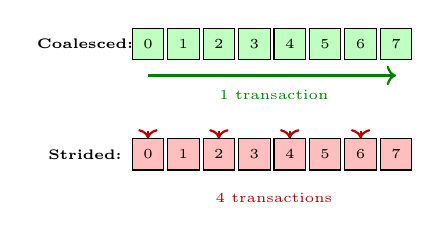
\begin{tikzpicture}[
                cell/.style={draw, minimum width=4mm, minimum height=4mm,
                             font=\tiny, inner sep=0pt},
                good/.style={cell, fill=green!25},
                bad/.style={cell, fill=red!25},
                lbl/.style={font=\tiny\bfseries},
            ]
                % Coalesced access
                \node[lbl] at (-0.8, 0) {Coalesced:};
                \foreach \i in {0,...,7} {
                    \node[good] at (\i*0.45, 0) {\i};
                }
                \draw[->, thick, green!50!black] (0, -0.4) -- (3.15, -0.4);
                \node[font=\tiny, green!50!black] at (1.6, -0.65) {1 transaction};

                % Strided access
                \node[lbl] at (-0.8, -1.4) {Strided:};
                \foreach \i in {0,...,7} {
                    \node[bad] at (\i*0.45, -1.4) {\i};
                }
                \foreach \i in {0,2,4,6} {
                    \draw[->, thick, red!70!black] (\i*0.45, -1.1) -- (\i*0.45, -1.2);
                }
                \node[font=\tiny, red!70!black] at (1.6, -1.95) {4 transactions};
            \end{tikzpicture}
            \end{center}
        \end{column}
    \end{columns}
\end{frame}

\begin{frame}{Asynchronous Memory Copying}
    \textbf{Host $\rightarrow$ Device DMA:}
    \begin{itemize}
        \item GPU DMA engines transfer over PCIe/NVLink without CPU
        \item \texttt{cudaMemcpyAsync()} for non-blocking transfers
        \item Requires page-locked (pinned) host buffers
    \end{itemize}

    \vspace{0.5em}
    \textbf{Device-Side Global $\rightarrow$ Shared:}
    \begin{itemize}
        \item \texttt{cp.async} or \texttt{cuda::memcpy\_async}
        \item Data movement decoupled from warp execution
    \end{itemize}

    \vspace{0.5em}
    \textbf{Pipelining \& Overlap:}
    \begin{itemize}
        \item Multi-stage pipelines (double-buffering)
        \item Issue next-tile copies before consuming current
        \item Hides hundreds of cycles of global-memory latency
    \end{itemize}

    \vspace{0.5em}
    \textbf{Best Practices:}
    \begin{itemize}
        \item Use \texttt{cudaHostAlloc} for true async DMA
        \item Align data to cache-line boundaries
    \end{itemize}
\end{frame}

\begin{frame}[fragile]{Pipelining with Latency Hiding (1/2)}
\begin{lstlisting}[escapeinside={(*@}{@*)}]
template <size_t stages_count = 2 (*@\tikzmark{stages}@*)/* Pipeline with stages_count stages */>
__global__ void with_staging_unified(int* global_out, int const* global_in,
                                     size_t size, size_t batch_sz) {
    auto grid = cooperative_groups::this_grid();
    auto block = cooperative_groups::this_thread_block();
    assert(size == batch_sz * grid.size()); // Assume input size fits batch_sz * grid_size

    extern __shared__ int shared[];(*@\tikzmark{shared}@*) // stages_count * block.size() * sizeof(int) bytes
    size_t shared_offset[stages_count];
    for (int s = 0; s < stages_count; ++s) shared_offset[s] = s * block.size();

    __shared__ cuda::pipeline_shared_state<(*@\tikzmark{pipestate}@*)
        cuda::thread_scope::thread_scope_block,
        stages_count
    > shared_state;
    auto pipeline = cuda::make_pipeline(block, &shared_state);(*@\tikzmark{makepipe}@*)

    auto block_batch = [&](size_t batch) -> int {
        return block.group_index().x * block.size() + grid.size() * batch;
    };
\end{lstlisting}
\begin{tikzpicture}[remember picture, overlay,
    callout/.style={rectangle callout, draw=blue!70, fill=blue!10,
                    font=\tiny, callout absolute pointer={#1},
                    rounded corners=2pt, text width=22mm, align=center}]
    \only<2->{
    \node[callout={(pic cs:stages)}, anchor=south] at ([shift={(0mm,3mm)}]pic cs:stages)
        {Double buffering\\(2 stages)};
    \node[callout={(pic cs:shared)}, anchor=west] at ([shift={(50mm,0mm)}]pic cs:shared)
        {Staging buffers\\in shared memory};
    \node[callout={(pic cs:pipestate)}, anchor=west] at ([shift={(50mm,0mm)}]pic cs:pipestate)
        {Pipeline state for\\block synchronization};
    }
\end{tikzpicture}
\end{frame}

\begin{frame}[fragile]{Pipelining with Latency Hiding (2/2)}
\begin{lstlisting}[escapeinside={(*@}{@*)}]
    // compute_batch: next batch to process
    // fetch_batch:  next batch to fetch from global memory
    for (size_t compute_batch = 0, fetch_batch = 0;(*@\tikzmark{twoptr}@*) compute_batch < batch_sz;
         ++compute_batch) {
        // The outer loop iterates over the computation of the batches
        for (; fetch_batch < batch_sz && fetch_batch < (compute_batch + stages_count);(*@\tikzmark{keepfull}@*)
             ++fetch_batch) {
            // This inner loop iterates over the memory transfers,
            // making sure that the pipeline is always full
            pipeline.producer_acquire();(*@\tikzmark{produce}@*)
            size_t shared_idx = fetch_batch % stages_count;(*@\tikzmark{modulo}@*)
            size_t batch_idx = fetch_batch;
            size_t block_batch_idx = block_batch(batch_idx);
            cuda::memcpy_async(block, shared + shared_offset[shared_idx],(*@\tikzmark{async}@*)
                               global_in + block_batch_idx,
                               sizeof(int) * block.size(), pipeline);
            pipeline.producer_commit();
        }
        pipeline.consumer_wait();(*@\tikzmark{consume}@*)
        int shared_idx = compute_batch % stages_count;
        int batch_idx = compute_batch;
        compute(global_out + block_batch(batch_idx), shared + shared_offset[shared_idx]);
        pipeline.consumer_release();
    }
\end{lstlisting}
\begin{tikzpicture}[remember picture, overlay,
    callout/.style={rectangle callout, draw=blue!70, fill=blue!10,
                    font=\tiny, callout absolute pointer={#1},
                    rounded corners=2pt, text width=24mm, align=center}]
    \only<2->{
    \node[callout={(pic cs:twoptr)}, anchor=south] at ([shift={(0mm,3mm)}]pic cs:twoptr)
        {Two pointers:\\fetch ahead of compute};
    \node[callout={(pic cs:keepfull)}, anchor=south west] at ([shift={(3mm,2mm)}]pic cs:keepfull)
        {Keep pipeline full\\(fetch up to stages\_count ahead)};
    \node[callout={(pic cs:produce)}, anchor=west] at ([shift={(45mm,0mm)}]pic cs:produce)
        {Producer: acquire slot,\\async copy, commit};
    \node[callout={(pic cs:consume)}, anchor=west] at ([shift={(45mm,0mm)}]pic cs:consume)
        {Consumer: wait for data,\\compute, release slot};
    }
\end{tikzpicture}
\end{frame}

\begin{frame}{Unified Memory}
    \textbf{Single, shared address space between CPU and GPU.}

    \vspace{0.5em}
    \textbf{Features:}
    \begin{itemize}
        \item Both processors transparently access the same data
        \item Automatically migrates pages on-demand
        \item Enables memory overcommitment
    \end{itemize}

    \vspace{1em}
    \textbf{Considerations:}
    \begin{itemize}
        \item No hardware coherence
        \item All SM translations blocked until page-fault handled
    \end{itemize}

    \vspace{0.5em}
    \textbf{Best Practices:}
    \begin{itemize}
        \item For predictable access patterns, issue prefetch hints
        \item Pin or allocate performance-critical buffers explicitly
    \end{itemize}
\end{frame}

%===============================================================================
\section{GPU I/O}
%===============================================================================

\begin{frame}{GPGPU I/O Challenges}
    \textbf{CPU--GPU link is often a bottleneck.}

    \vspace{0.5em}
    \begin{columns}
        \begin{column}{0.5\textwidth}
            \textbf{Compute (B200):}
            \begin{itemize}
                \item $\sim$2.2 PFLOP/s (FP16 Tensor)
                \item On-GPU Bandwidth: 8 TB/s
            \end{itemize}

            \vspace{0.5em}
            \textbf{Links:}
            \begin{itemize}
                \item PCIe 5.0 $\times$16: $\sim$126 GB/s
                \item NVLink 5 (Blackwell): 1.8 TB/s
            \end{itemize}
        \end{column}
        \begin{column}{0.5\textwidth}
            \textbf{Overheads:}
            \begin{itemize}
                \item Data transfer to/from CPU
                \item CPU involvement for disk/network I/O
                \item Synchronous I/O operations
            \end{itemize}

            \vspace{0.5em}
            \textbf{Storage:}
            \begin{itemize}
                \item NVMe SSD: 3--7 GB/s
            \end{itemize}
        \end{column}
    \end{columns}

    \vspace{1em}
    \begin{block}{Key Insight}
        Many workloads choke on data movement and delivery.
    \end{block}

    {\scriptsize Source: NVIDIA B200 Datasheet, GTC 2024}
\end{frame}

\begin{frame}{GPUDirect Storage}
    \textbf{Direct NVMe/NVMe-oF to GPU path --- bypasses CPU memory.}\\
    \textbf{GPUDirect RDMA}: Network-to-GPU without CPU involvement.\\
    {\small Without GPUDirect: CPU memory controller orchestrates two-stage copy.}

    \begin{center}
    \begin{tikzpicture}[
        node distance=15mm,
        icon/.style={inner sep=0pt},
        lbl/.style={font=\scriptsize\bfseries},
        link/.style={draw=gray!60, thick},
        bounce/.style={draw=red!70, very thick, ->},
        gds/.style={draw=green!60!black, very thick, ->},
    ]
        % === Left side: Without GPUDirect Storage ===
        \node[font=\scriptsize\bfseries] (title1) {Without GPUDirect Storage};
        \node[icon, below=5mm of title1, label={[lbl]above:Switch}] (sw1)
            {\includegraphics[height=10mm]{figures/noun-switch-7787836.png}};
        \node[icon, left of=sw1, label={[lbl]above:CPU}] (cpu1)
            {\includegraphics[height=8mm]{figures/noun-cpu-8157304.png}};
        \node[icon, below of=cpu1, label={[lbl]below:Memory}] (mem1)
            {\includegraphics[height=8mm]{figures/06-ram-dimm-icon.png}};
        \node[icon, right of=sw1, label={[lbl]above:NVMe}] (nvme1)
            {\includegraphics[height=5mm]{figures/noun-nvme-5566039.png}};
        \node[icon, below of=sw1, label={[lbl]below:GPU}] (gpu1)
            {\includegraphics[height=10mm]{figures/noun-gpu-8141519.png}};

        % Connections - left side
        \draw[link] (cpu1) -- (mem1);
        \draw[link] (cpu1) -- (sw1);
        \draw[link] (sw1) -- (nvme1);
        \draw[link] (sw1) -- (gpu1);
        % Bounce buffer path (red) - two stages via CPU (memory controller)
        % Stage 1: NVMe -> CPU -> Memory
        \draw[bounce, transform canvas={yshift=2pt}] (nvme1.west) to[out=180,in=0] (cpu1.east);
        \draw[bounce, transform canvas={xshift=-2pt}] (cpu1.south) -- (mem1.north);
        % Stage 2: Memory -> CPU -> GPU (upside-down U)
        \draw[bounce, transform canvas={xshift=2pt}] (mem1.north) to[out=90,in=180] (cpu1.east)
            to[out=0,in=90] (gpu1.north);

        % === Right side: With GPUDirect Storage ===
        \begin{scope}[xshift=55mm]
            \node[font=\scriptsize\bfseries] (title2) {With GPUDirect Storage};
            \node[icon, below=5mm of title2, label={[lbl]above:Switch}] (sw2)
                {\includegraphics[height=10mm]{figures/noun-switch-7787836.png}};
            \node[icon, left of=sw2, label={[lbl]above:CPU}] (cpu2)
                {\includegraphics[height=8mm]{figures/noun-cpu-8157304.png}};
            \node[icon, below of=cpu2, label={[lbl]below:Memory}] (mem2)
                {\includegraphics[height=8mm]{figures/06-ram-dimm-icon.png}};
            \node[icon, right of=sw2, label={[lbl]above:NVMe}] (nvme2)
                {\includegraphics[height=5mm]{figures/noun-nvme-5566039.png}};
            \node[icon, below of=sw2, label={[lbl]below:GPU}] (gpu2)
                {\includegraphics[height=10mm]{figures/noun-gpu-8141519.png}};

            % Connections - right side (inactive shown lighter)
            \draw[link, opacity=0.3] (cpu2) -- (mem2);
            \draw[link, opacity=0.3] (cpu2) -- (sw2);
            % GPUDirect path (green, direct)
            \draw[gds] (nvme2) -- (sw2);
            \draw[gds] (sw2) -- (gpu2);

            % Legend in bottom-right
            \node[anchor=north west, font=\scriptsize, align=left, right=5mm of gpu2] {
                \tikz[baseline=-0.5ex]\draw[red!70, very thick, ->] (0,0) -- (5mm,0); Bounce\\[1pt]
                \tikz[baseline=-0.5ex]\draw[green!60!black, very thick, ->] (0,0) -- (5mm,0); GPUDirect
            };
        \end{scope}
    \end{tikzpicture}
    \end{center}

    \textbf{Performance:} Up to 50 GB/s with GPUDirect Storage
\end{frame}

\begin{frame}{Multi-Instance GPU (MIG)}
    \begin{columns}
        \begin{column}{0.5\textwidth}
            \textbf{Isolation and QoS mechanism.}

            \vspace{0.5em}
            \textbf{Each instance gets its own:}
            \begin{itemize}
                \item Compute cores
                \item On-chip memory and cache
                \item Memory bandwidth
            \end{itemize}

            \vspace{0.5em}
            \textbf{Features:}
            \begin{itemize}
                \item Partitioned into different-sized instances
                \item Dynamically reconfigurable
                \item Strong isolation between workloads
            \end{itemize}

            \vspace{0.5em}
            \textbf{Limitations:}
            \begin{itemize}
                \item Limited number of instances
                \item Resources proportionally fixed
            \end{itemize}
        \end{column}
        \begin{column}{0.5\textwidth}
            \begin{center}
            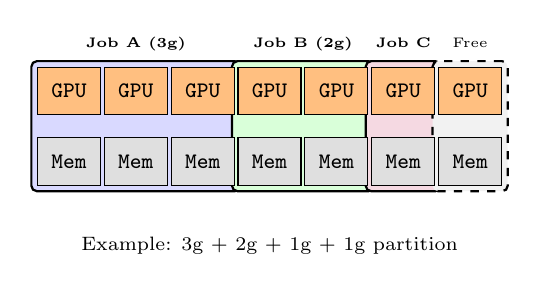
\begin{tikzpicture}[
                slice/.style={draw, minimum width=8mm, minimum height=6mm, font=\footnotesize\ttfamily},
                gpu/.style={slice, fill=orange!50},
                mem/.style={slice, fill=gray!25},
                grp/.style={draw, thick, rounded corners=2pt, inner sep=2pt},
                joblbl/.style={font=\tiny\bfseries, text depth=0.25ex},
            ]
                % GPU slices row
                \matrix[matrix of nodes, nodes={gpu}, column sep=1pt, row sep=1pt,
                        ampersand replacement=\&] (gpus) {
                    GPU \& GPU \& GPU \& GPU \& GPU \& GPU \& GPU \\
                };
                % Memory slices row
                \matrix[matrix of nodes, nodes={mem}, column sep=1pt, row sep=1pt,
                        ampersand replacement=\&, below=1pt of gpus] (mems) {
                    Mem \& Mem \& Mem \& Mem \& Mem \& Mem \& Mem \\
                };

                % Workload grouping boxes on background layer
                \begin{scope}[on background layer]
                    \node[grp, fill=blue!15, fit=(gpus-1-1) (gpus-1-3) (mems-1-1) (mems-1-3),
                          label={[joblbl]above:Job A (3g)}] {};
                    \node[grp, fill=green!15, fit=(gpus-1-4) (gpus-1-5) (mems-1-4) (mems-1-5),
                          label={[joblbl]above:Job B (2g)}] {};
                    \node[grp, fill=purple!15, fit=(gpus-1-6) (mems-1-6),
                          label={[joblbl]above:Job C}] {};
                    \node[grp, fill=gray!10, dashed, fit=(gpus-1-7) (mems-1-7),
                          label={[font=\tiny, text depth=0.25ex]above:Free}] {};
                \end{scope}

                % Label
                \node[below=4mm of mems, font=\scriptsize] {Example: 3g + 2g + 1g + 1g partition};
            \end{tikzpicture}
            \end{center}
        \end{column}
    \end{columns}
\end{frame}

%===============================================================================
\section{Summary}
%===============================================================================

\begin{frame}{Summary}
    \begin{itemize}
        \item \textbf{GPGPU}: Massive parallelism for data-parallel workloads
        \item \textbf{Roofline Model}: Analyze compute vs memory-bound kernels
        \item \textbf{Warp Scheduling}: Latency hiding through occupancy
        \item \textbf{Divergence}: Avoid branches within warps
        \item \textbf{Tensor Cores}: Accelerated matrix operations (FP16, BF16, TF32)
        \item \textbf{HBM}: High-bandwidth memory (3+ TB/s)
        \item \textbf{Async Memory}: Overlap compute and data movement
        \item \textbf{GPUDirect}: Bypass CPU for storage and network I/O
        \item \textbf{MIG}: Partition GPU for isolation and QoS
    \end{itemize}

    \vspace{1em}
    \begin{block}{Conclusion}
        GPUs provide massive parallelization with unique challenges in compute (divergence) and I/O (limited links). They are increasingly becoming ``first-class citizens'' in modern computing.
    \end{block}
\end{frame}

\end{document}
